Se implemento una simulación en Python para observar los efectos del muestreo
instantáneo y natural sobre señales analógicas. El código desarrollado permite
observar que sucede en cada etapa del proceso de muestreo, ademas de tener
la capacidad de poder saltear etapas y observar los efectos de cada una, tanto 
en el dominio del tiempo como en el de la frecuencia.

El código se implemento en Python utilizando las librerías numpy, scipy, matplotlib,
y PyQt5. La interfaz gráfica permite decidir con que señal de entrada se quiere
trabajar, la frecuencia de muestreo, el tipo de muestreo (instantáneo o natural),
y la frecuencia de corte de los filtro anti-alias y de reconstrucción.
Tabién permite variar el duty cycle del sample and hold.
Ambos filtros (anti-alias y de reconstrucción) se implenetaron
usando la funcion de aproximación de Cauer (elliptic) de orden 6,
al igual que en la placa del circuito impreso.
Además, indica con puntos naranjas donde se muestreó la señal de entrada
A continuación se muestran algunas capturas de pantalla de la interfaz gráfica:

\begin{figure}[H]
    \centering
    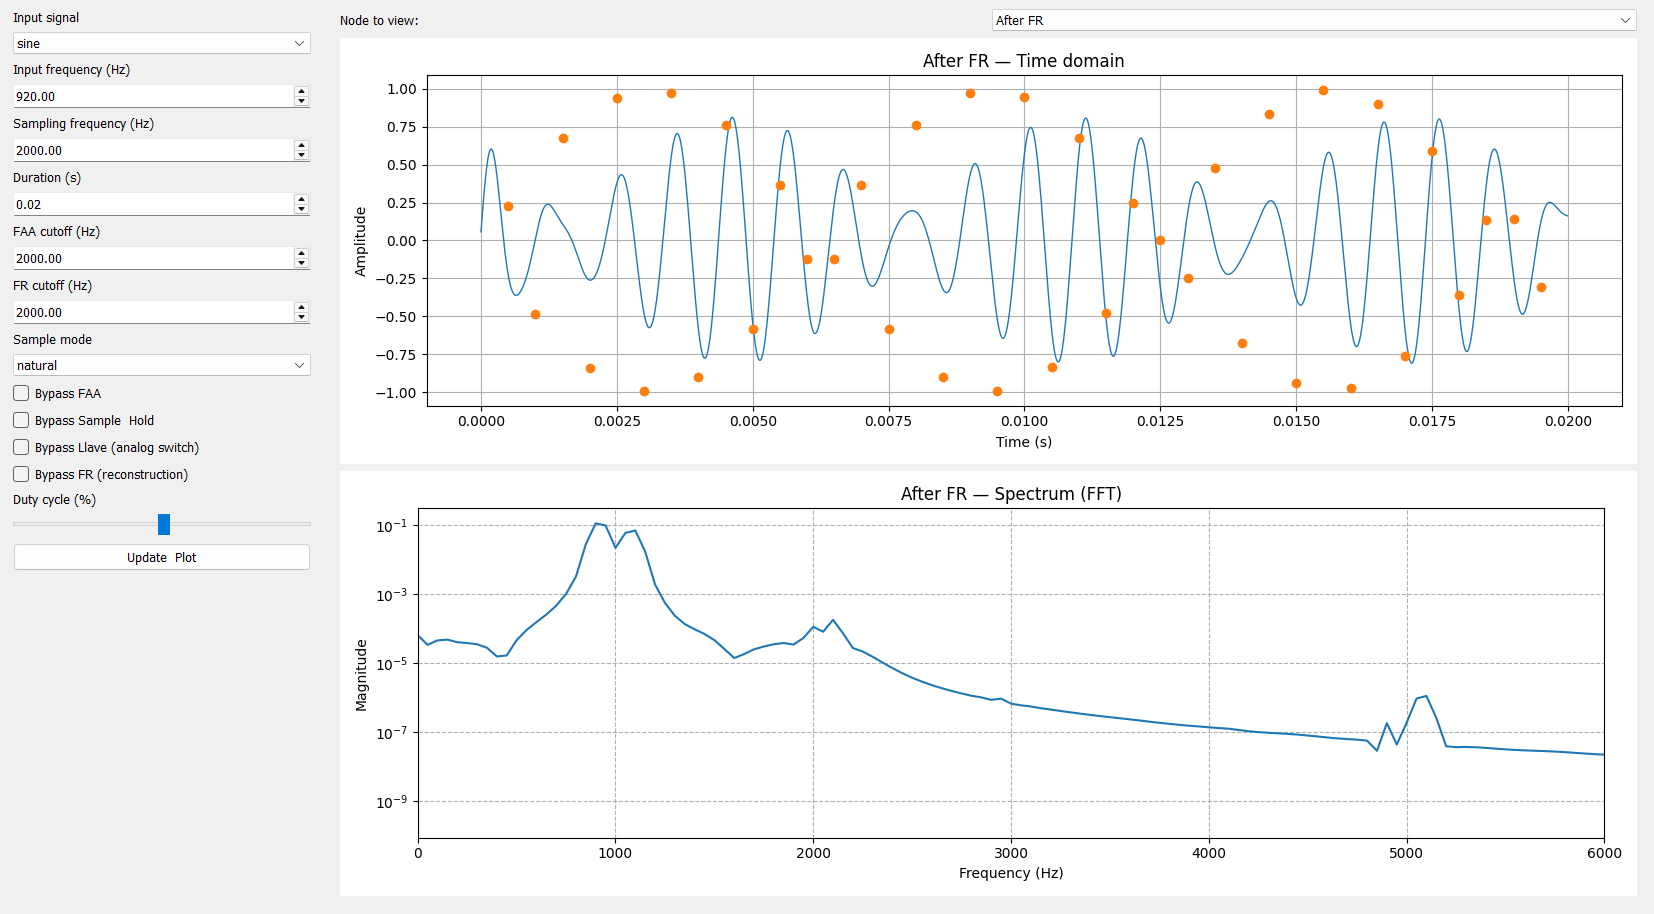
\includegraphics[width=0.8\textwidth]{Imagenes/gui_beating.png}
    \caption{Interfaz gráfica - Ejemplo de señal en la GUI}
    \label{fig:interfaz1}
\end{figure}

Donde se puede apreciar el efecto de ``beating'' ya que el la señal de entrada
es cercana a $f_s/2$, el filtro recuperador no es capaz de eliminar el aliasing
y se observa una señal modulada en amplitud.
\\\\Todo el codigo fuente se encuentra en el repositorio de GitHub: \ref{Git}

